\documentclass[12pt]{article}
\usepackage{graphicx}
\usepackage{float}
\usepackage{hyperref}
\usepackage{tfrupee}
\usepackage{ragged2e}
\usepackage{multicol}
\usepackage{multirow}
\usepackage{xurl}
\usepackage{geometry}
\usepackage{mathtools}
\usepackage{enumitem}
\DeclarePairedDelimiter\ceil{\lceil}{\rceil}
\DeclarePairedDelimiter\floor{\lfloor}{\rfloor}
 \geometry{
 a4paper,
 total={170mm,240mm},
 left=20mm,
 top=20mm,
 }
% begin the document.
\begin{document}

% make a title page.[this creates title page]
\begin{center}\textbf{
\LARGE{EE338 : Digital Signal Processing}\\\vspace{1em}
\vspace{1em} \\ 
\LARGE{Filter Design Assignment II}\\
\vspace{1em}
\large{March 10, 2023}\\
\vfill
\begin{figure}[H]
    \centering
    \includegraphics[scale = 0.2]{logo.png}
\end{figure}
\vspace{1em}
\large{Indian Institute of Technology, Bombay}\\
\vfill
\LARGE{Amruta Mahendra Parulekar} \\
\LARGE{Roll no. 20d070009} \vspace{2em}
\\\large{Reviewed by Harshvardhan, 20d070035}

}
\end{center}

\newpage
\tableofcontents
\newpage
\section{Student Details} %[This segment creates Section as seen in document]
\begin{itemize}[nolistsep]
    \item Name = Amruta Mahendra Parulekar
    \item Roll no. = 20d070009
    \item Filter number m = 26
    \item Group number = 3
    \item Review member = Harshvardhan, 20d070035 (Has reviewed my report)
\end{itemize}
\section{Chebyshev filter Design}
\subsection{Un-normalized discrete time filter specifications}

  
    The filter to be designed is a Band-stop filter where:
    \begin{equation}
        q(m) = \floor{m/10} = \floor{2.6} = 2
    \end{equation}
    \begin{equation}
        r(m) = 26 - 10*q(m) = 26 - 10*2 = 6
    \end{equation}
    \begin{equation}
        BL(m) = 20 + 3*q(m) + 11*r(m) = 20 + 3*2 + 11*6 = 92
    \end{equation}
    \begin{equation}
        BH(m) = BL(m) + 40 = 92 + 40 = 132
    \end{equation}
  

    \begin{enumerate}
    \item \textbf{The passband will be equiripple and the stopband will be monotonic}
    \item \textbf{The stopband will be from 92 kHz to 132 kHz}
    \item \textbf{The transition band will be 5 kHz on either side of the stopband}
    \item \textbf{The passband is from 0 - 87 kHz and 137 - 212.5kHz} ( sampling rate 425 kHz)
    \item \textbf{The passband and stopband tolerances are 0.15 in magnitude}

\end{enumerate}
\subsection{Normalized discrete time filter specifications}
Sampling rate is 425 kHz, which corresponds to 2$\pi$ on the normalized frequency axis.
\\So on normalizing the frequency axis, each frequency $\Omega_1$ below 212.5 kHz gets mapped using the function:
\begin{equation}
    \omega=\frac{\Omega_1 * 2 \pi}{(Sampling Rate)}
\end{equation}
\begin{enumerate}
    \item \textbf{The passband will be equiripple and the stopband will be monotonic}
    \item \textbf{The stopband will be from 0.4329 $\pi$ to 0.6212 $\pi$}
    \item \textbf{The transition band will be 0.0235 $\pi$ on either side of the stopband}
    \item \textbf{The passband will be from 0 - 0.4094 $\pi$ and 0.6447 $\pi$ - $\pi$} 
    \item \textbf{The passband and stopband tolerances are 0.15 in magnitude}

\end{enumerate}
\newpage
\subsection{Analog filter specifications }
The discrete time filter specifications can be converted to corresponding analog filter specifications by using a bilinear transform, which is given as:
\begin{equation}
    \Omega = tan(\omega/2)
\end{equation}
\begin{enumerate}
    \item \textbf{The passband will be equiripple and the stopband will be monotonic}
    \item \textbf{The stopband will be from 0.8086 ($\Omega_{s1}$) to 1.4774($\Omega_{s2}$)}
    \item \textbf{The transition band will be from 0.7493 ($\Omega_{p1}$) - 0.8086 ($\Omega_{s1}$) and \\1.4774($\Omega_{s2}$) - 1.6018 ($\Omega_{p2}$)}
    \item \textbf{The passband will be from 0 - 0.7493 ($\Omega_{p1}$)  and 1.6018 ($\Omega_{p2}$) - infinity} 
    \item \textbf{The passband and stopband tolerances are 0.15 in magnitude}
\end{enumerate}
\subsection{The frequency transformation }
We use the bandstop transformation to convert the band pass filter to a lower filter:
\begin{equation}
    \Omega_L=\frac{B\Omega}{\Omega_{0}^2-\Omega^2}
\end{equation}
The two parameters B and $\Omega_{0}$ are obtained by the relations:
\begin{equation}
    \Omega_{0}=\sqrt{\Omega_{p1}*\Omega_{p2}}= \sqrt{0.7493*1.6108}=1.099
    \end{equation}
    \begin{equation}   
    B=\Omega_{p2}-\Omega_{p1}=0.8615
 \end{equation}
 \begin{center}
\def\arraystretch{1.1}
\bgroup
\begin{tabular}{|c|c|}
\hline
\textbf{$\Omega$ }
& \textbf{$\Omega_L$ }\\ 
\hline \hline
$0^+$  &  $0^+$  \\ 
\hline 
0.7493 ($\Omega_{p1}$)   &   +1 ($\Omega_{Lp1}$) \\ 
\hline
0.8086 ($\Omega_{s1}$)  &   1.2578  ($\Omega_{Ls1}$)\\ 
\hline
1.099  ($\Omega_{0-}$) & +infinity  \\ 
\hline
1.099  ($\Omega_{0+}$) & -infinity  \\ 
\hline
1.4774 ($\Omega_{s2}$)   &  -1.3029 ($\Omega_{Ls2}$) \\ 
\hline
1.6108 ($\Omega_{p2}$)  &   -1 ($\Omega_{Lp2}$) \\ 
 \hline
 infinity & $0^-$ \\
 \hline
\end{tabular}
\egroup
\end{center}
\subsection{Frequency transformed lowpass analog filter specifications}
\begin{enumerate}
    \item \textbf{The passband will be equiripple and the stopband will be monotonic}
    \item \textbf{The passband edge will be at 1($\Omega_{Lp}$)}
    \item \textbf{The stopband edge will be min($\Omega_{Ls1}$,$-\Omega_{Ls2}$) which is 1.2578($\Omega_{Ls}$)}
    \item \textbf{The passband and stopband tolerances are 0.15 in magnitude}

\end{enumerate}
\newpage
\subsection{The analog lowpass filter transfer function}
We require a Chebyshev Bandpass filter, which means that  the passband is equiripple and stopband is monotonic.
\\Since the tolerance ($\delta$) in both passband and stopband is 0.15, we define :
\begin{equation}
    D1= \frac{1}{(1-\delta)^2}-1 = 0.3841
\end{equation}
\begin{equation}
    D2= \frac{1}{(\delta)^2}-1 = 43.444
\end{equation}
The inequality for the order N of the Chebyshev filter is:
\begin{equation}
    N_{min}=\ceil{\frac{cosh^{-1}(\sqrt{D2/D1})}{cosh^{-1}(\Omega_{Ls}/\Omega_{Lp})}} = 5
\end{equation}
The parameter $\epsilon$ is chosen to be $\sqrt{D_1}$
\\The poles of the transfer function can be obtained by solving:
\begin{equation}
   1+ D_1cosh^2(N_{min}cosh^{-1}(\frac{s}{j})) = 1+ 0.3841cosh^2(5cosh^{-1}(\frac{s}{j})) = 0
\end{equation}
On plotting the above equation, we get the location of the roots using Wolfram alpha as shown:
\begin{figure}[H]
    \centering
    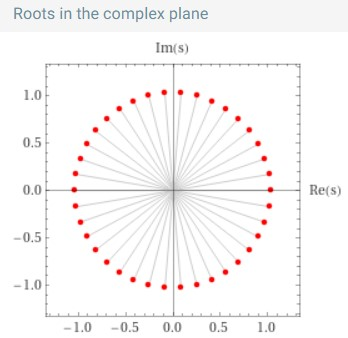
\includegraphics[]{poles.jpg}
\end{figure}

The poles obtained are symmetric about the origin and we can pick one from each pair for our transfer function. We choose poles from the LHCP to allow stability. 
\newpage
The poles chosen are:
\begin{figure}[H]
    \centering
    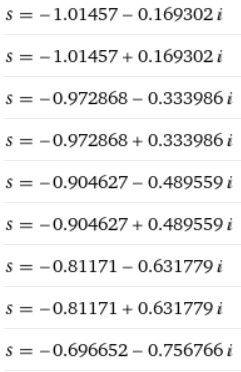
\includegraphics[]{roots.jpg}
   \\ 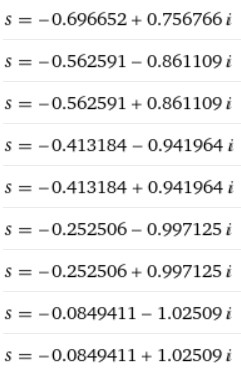
\includegraphics[]{r2.jpg}
\end{figure}
As N=odd, we can write the transfer function as:
\begin{equation}
    H_{analog,LPF}(s_L)=\frac{\prod_{i=0}^{4}(-p_i)}{\prod_{i=0}^{4
    }(s_L-p_i)}
\end{equation}
The numerator has been scaled to get a DC gain of 1.
\subsection{The analog bandstop filter transfer function}
The transformation equation:
\begin{equation}
    s_L= \frac{Bs}{s^2+\Omega_{0}^2} = \frac{0.8615*s}{s^2+1.2078}
\end{equation}
Thus, the transfer function:
\begin{equation}
    H_{analog,BSF}(s)=\frac{(s^2+\Omega_{0}^2)^5}{\prod_{i=0}^{4}(s^2-\frac{Bs}{p_i}+\Omega_{0}^2)} 
\end{equation}
The zeroes are at $s=\pm$ j $ \Omega_0 $
\\Factorizing the denominator to get new roots so that the denominator can be expressed as a product of 10 monomials, we get the new poles as:
\begin{equation}
    pol_i=\frac{\frac{B}{p_i}\pm \sqrt{(\frac{B}{p_i})^2-4\Omega_{0}^2}}{2}
\end{equation}
Thus the new analog filter transfer function where $pol_i$ are poles of the analog bandstop filter is:
\begin{equation}
    H_{analog,BSF}(s)=\frac{(s^2+\Omega_{0}^2)^5}{\prod_{i=0}^{9}(s-pol_i)} 
\end{equation}
\newpage
The transfer function and its coefficients after expansion can be seen as:
\\\textbf{Numerator}: $s^{10}+6.039s^8+14.5878s^6+17.6191s^4+10.6402s^2+2.5702$
\\\textbf{Denominator}: $s^{10}+4.3958s^9+12.1385s^8+31.3020s^7+41.1761s^6+67.4940s^5+49.7326s^4+45.6628s^3+21.3870s^2+9.3545s+2.5702$

\subsection{The discrete time filter transfer function}
The bilinear transform from analog to discrete domain is:
\begin{equation}
    \frac{1-z^{-1}}{1+z^{-1}}
\end{equation}
On substituting this s in equation for the analog Bandstop filter, we get:
\begin{equation}
    H_{discrete,BSF}(z)=\frac{((1+j\Omega_0)+(-1+j\Omega_0)z^{-1})^5((1-j\Omega_0)-(1+j\Omega_0)z^{-1})^5}{\prod_{i=0}^{9}((1-pol_i)-(1+pol_i)z^{-1})} 
\end{equation}
Thus we get new the poles at:
\begin{equation}
    z_i=\frac{1+pol_i}{1-pol_i}
\end{equation}
Thus we get new the roots (each is a repeated root, repeated 5 times) at:
\begin{equation}
    zer1=\frac{1+j\Omega_0}{1-j\Omega_0};zer2=\frac{1-j\Omega_0}{1+j\Omega_0}
\end{equation}
Since we have $p_i$ values for the analog lowpass filter, we can use equation (17) to get $pol_i$ values for the poles of the analog bandstop filter. 
\\Once we have the  $pol_i$ values for the poles of the analog bandstop filter, we can use equation (21) to compute the poles of the discrete bandstop filter. 
\\The transfer function and its coefficients after expansion can be seen as:
\\\textbf{Numerator:}$52.4565z^{-10}+49.3727z^{-9}+280.8707z^{-8}+200.990z^{-7}+580.6590z^{-6}+303.2470z^{-5}+580.6590z^{-4}+200.9900z^{-3}+280.8707z^{-2}+49.3727z^{-1}+52.4565$
\\\textbf{Denominator:}$−30.2047z^{-10}−8.8064z^{-9}+59.0804z^{-8}+70.8348z^{-7}+287.2631z^{-6}+239.4211z^{-5}+637.1617z^{-4}+317.0984z^{-3}+588.4527z^{-2}+185.4192z^{-1}+286.2139$
\vfill
\begin{center}
    

\textbf{THUS THE CHEBYSHEV IIR FILTER DESIGN ASSIGNMENT HAS BEEN COMPLETED.}
\end{center}
\newpage
\section{Plots}

    
\subsection{The magnitude vs unnormalized frequency plot:}
\begin{center}
\includegraphics[scale=0.8]{mag.png}
\end{center}
\subsection{The phase vs unnormalized frequency plot}
\begin{center}
\includegraphics[scale=0.8]{ph.png}
\end{center}
\subsection{Observations:}
\begin{enumerate}[noitemsep]
    \item {The passband is equiripple and the stopband is monotonic}
    \item {The stopband is from 92 kHz to 132 kHz}
    \item {The transition band is 5 kHz on either side of the stopband}
    \item {The passband is from 0 - 87 kHz and 137 - 212.5kHz}
    \item {The passband and stopband tolerances are 0.15 in magnitude}

\end{enumerate}
\subsection{The magnitude vs omega plot:}
\begin{center}
\includegraphics[scale=0.8]{mag2.png}
\end{center}
\subsection{The phase vs omega plot}
\begin{center}
\includegraphics[scale=0.8]{ph2.png}
\end{center}
\subsection{Observations:} We can clearly view the points 0.7493 ($\Omega_{p1}$);0.8086 ($\Omega_{s1}$);1.4774($\Omega_{s2}$);1.6018 ($\Omega_{p2}$)
\section{Code}
\subsection{Code for evaluating the analog filter response:}
\begin{center}
\includegraphics[scale=0.8]{c1.jpg}

\end{center}
\subsection{Code for plots:}
\begin{center}
\includegraphics[]{c2.jpg}
\\\includegraphics[]{c3.jpg}
\end{center}
\subsection{Code for printing coefficients:}
\begin{center}
\includegraphics[scale=0.9]{c4.jpg}
\end{center}
\section{Peer Review}
\textbf{I have reviewed the report of Sameep Chattopadhyay (20d070035) and have found it to be correct.} 
\\The filter design steps were completed and the phase and magnitude response plots were present. He has started from the un-normalised filter, then normalized it, then converted to an analog filter, which was converted to a lowpass filter, to which he applied a frequency transform and then reconverted it to a bandstop filter.
\\His final plot also matches the requirements at the start.


\end{document}
